\chapter{Integration Strategy} \label{chap2}

\section{Entry Criteria}
The Integration Testing can be carried out after the successful completion of the Unit Testing of the entire software. In addition the following points should be valid:

\begin{itemize}
	\item The project should be code-complete and all its major features should be already present
	\item The project should satisfy the memory requirements specified in the RASD
	\item The correct version of the software is moved into the integration testing environment
	\item Sanity testing is done and build is stable for further testing
	\item The Database should be ready and its tables are populated with initial data
\end{itemize}

\section{Elements to be Integrated}
Due to the early stage of development of the software and the resulting low level of complexity of the entire system, we decided to focus our integration testing only on the main components of the Business Logic, keeping in mind that the future evolution of the project will lead to the creation of a number of subcomponent inside these component, needed to make the system fully working. Following this decision, we are going to integrate the Web Component and the Business Logic Component, testing the direct connections between the managed Beans and their corresponding Managers and we are also going to integrate the 7 subcomponents of the Business Logic Component.

\section{Integration Testing Strategy}
Due to the particular stage of development explained in the previous point, at the moment there is not a complete hierarchy of (sub)components and (sub)systems, so it's not possible to fully define the integration test strategy followed in this document, because all the components involved are on the same level. Anyway the selected approach is the top-down approach, because (as stated in the previous point) in the future other lower level subcomponents will be implemented and then the testing will follow this downward development.

\section{Sequence of Component / Function Integration}

\begin{figure}[!htbp]
\centering
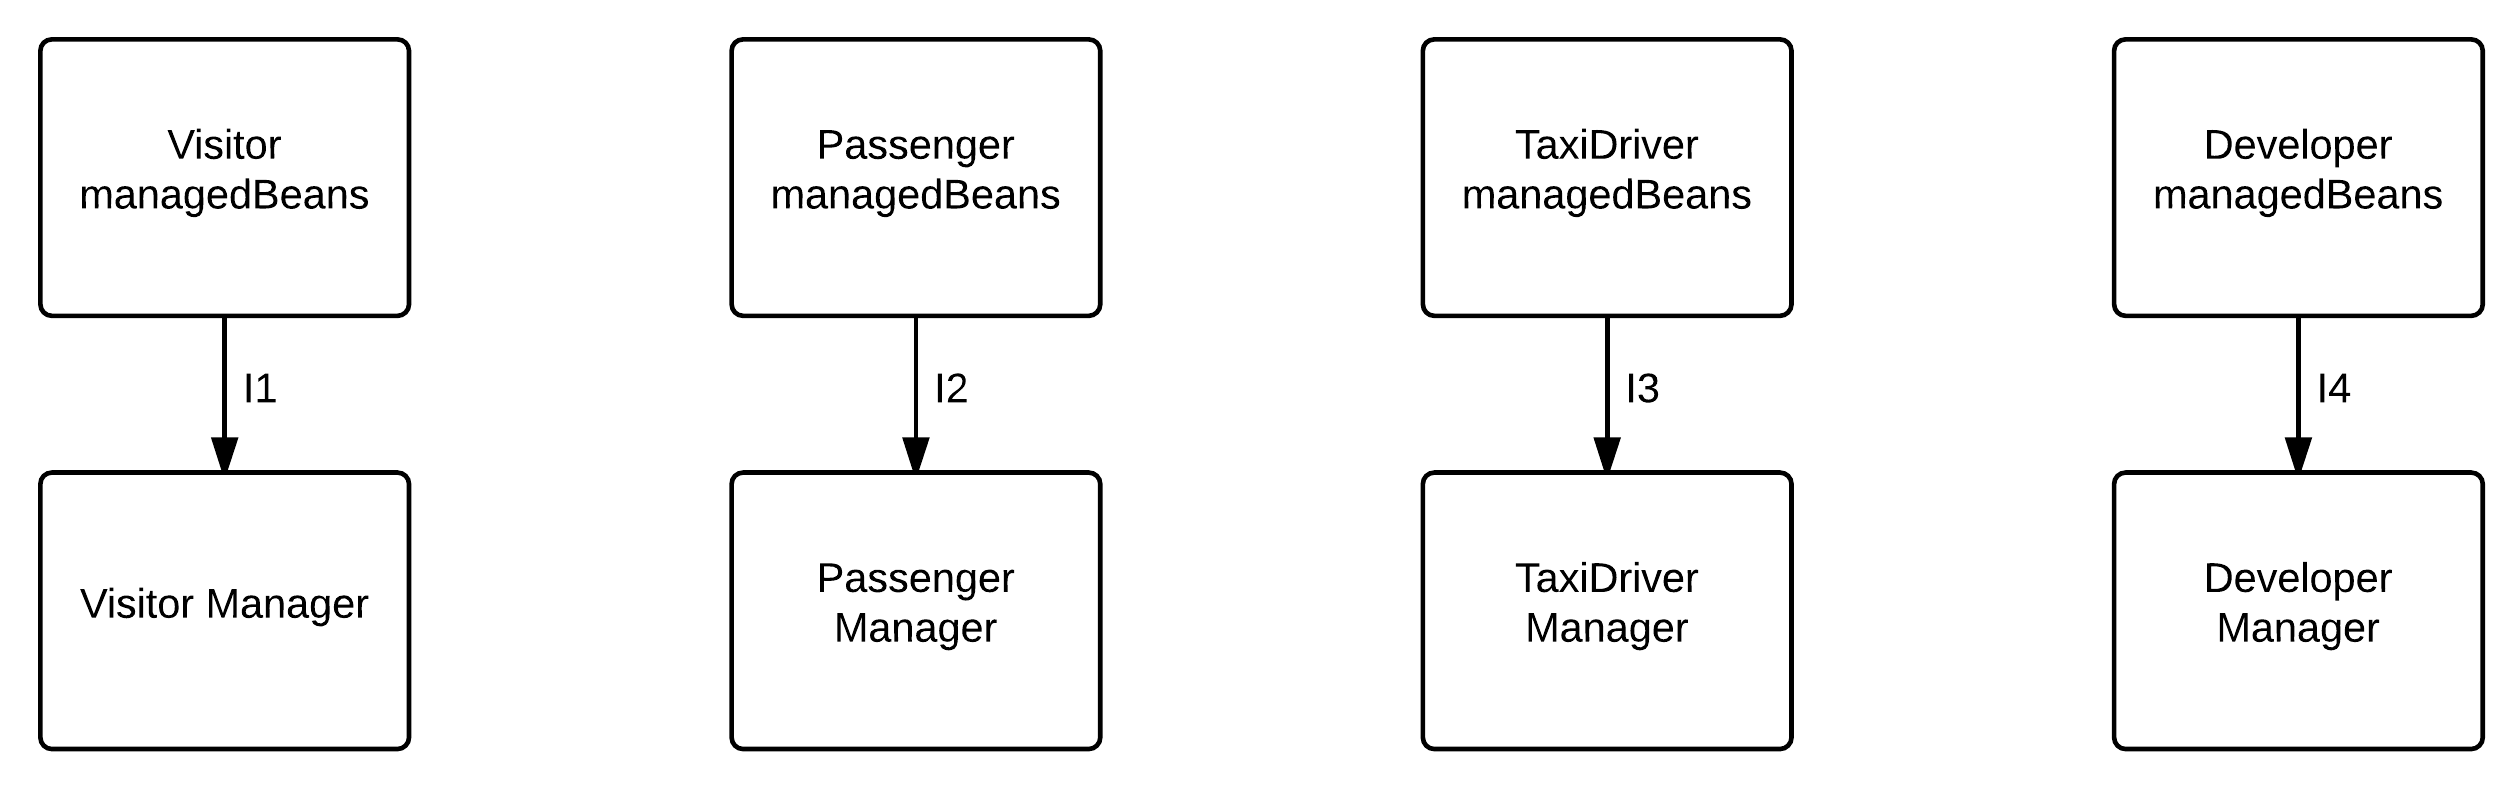
\includegraphics[width=\textwidth]{cpt/img/ITDPComponentDiagramsTP1}
\end{figure}

\begin{table}[!htbp]
\begin{center}
\begin{tabular}[t]{c|p{0.7\textwidth}|c}

\textbf{ID} & \textbf{Integration Test} & \textbf{Paragraphs} \\
\hline
I1 & Visitor managedBean $\rightarrow$ Visitor Manager & 3.1.1  3.2.1 \\
\hline
I2 & Passenger managedBean $\rightarrow$ Passenger Manager & 3.1.2  3.2.1 \\
\hline
I3 & TaxiDriver managedBean $\rightarrow$ TaxiDriver Manager & 3.1.3  3.2.1 \\
\hline
I4 & Developer managedBean $\rightarrow$ Developer Manager & 3.1.4  3.2.1 \\
\hline
\end{tabular}
\end{center}
\end{table}

\begin{figure}[!htbp]
\centering
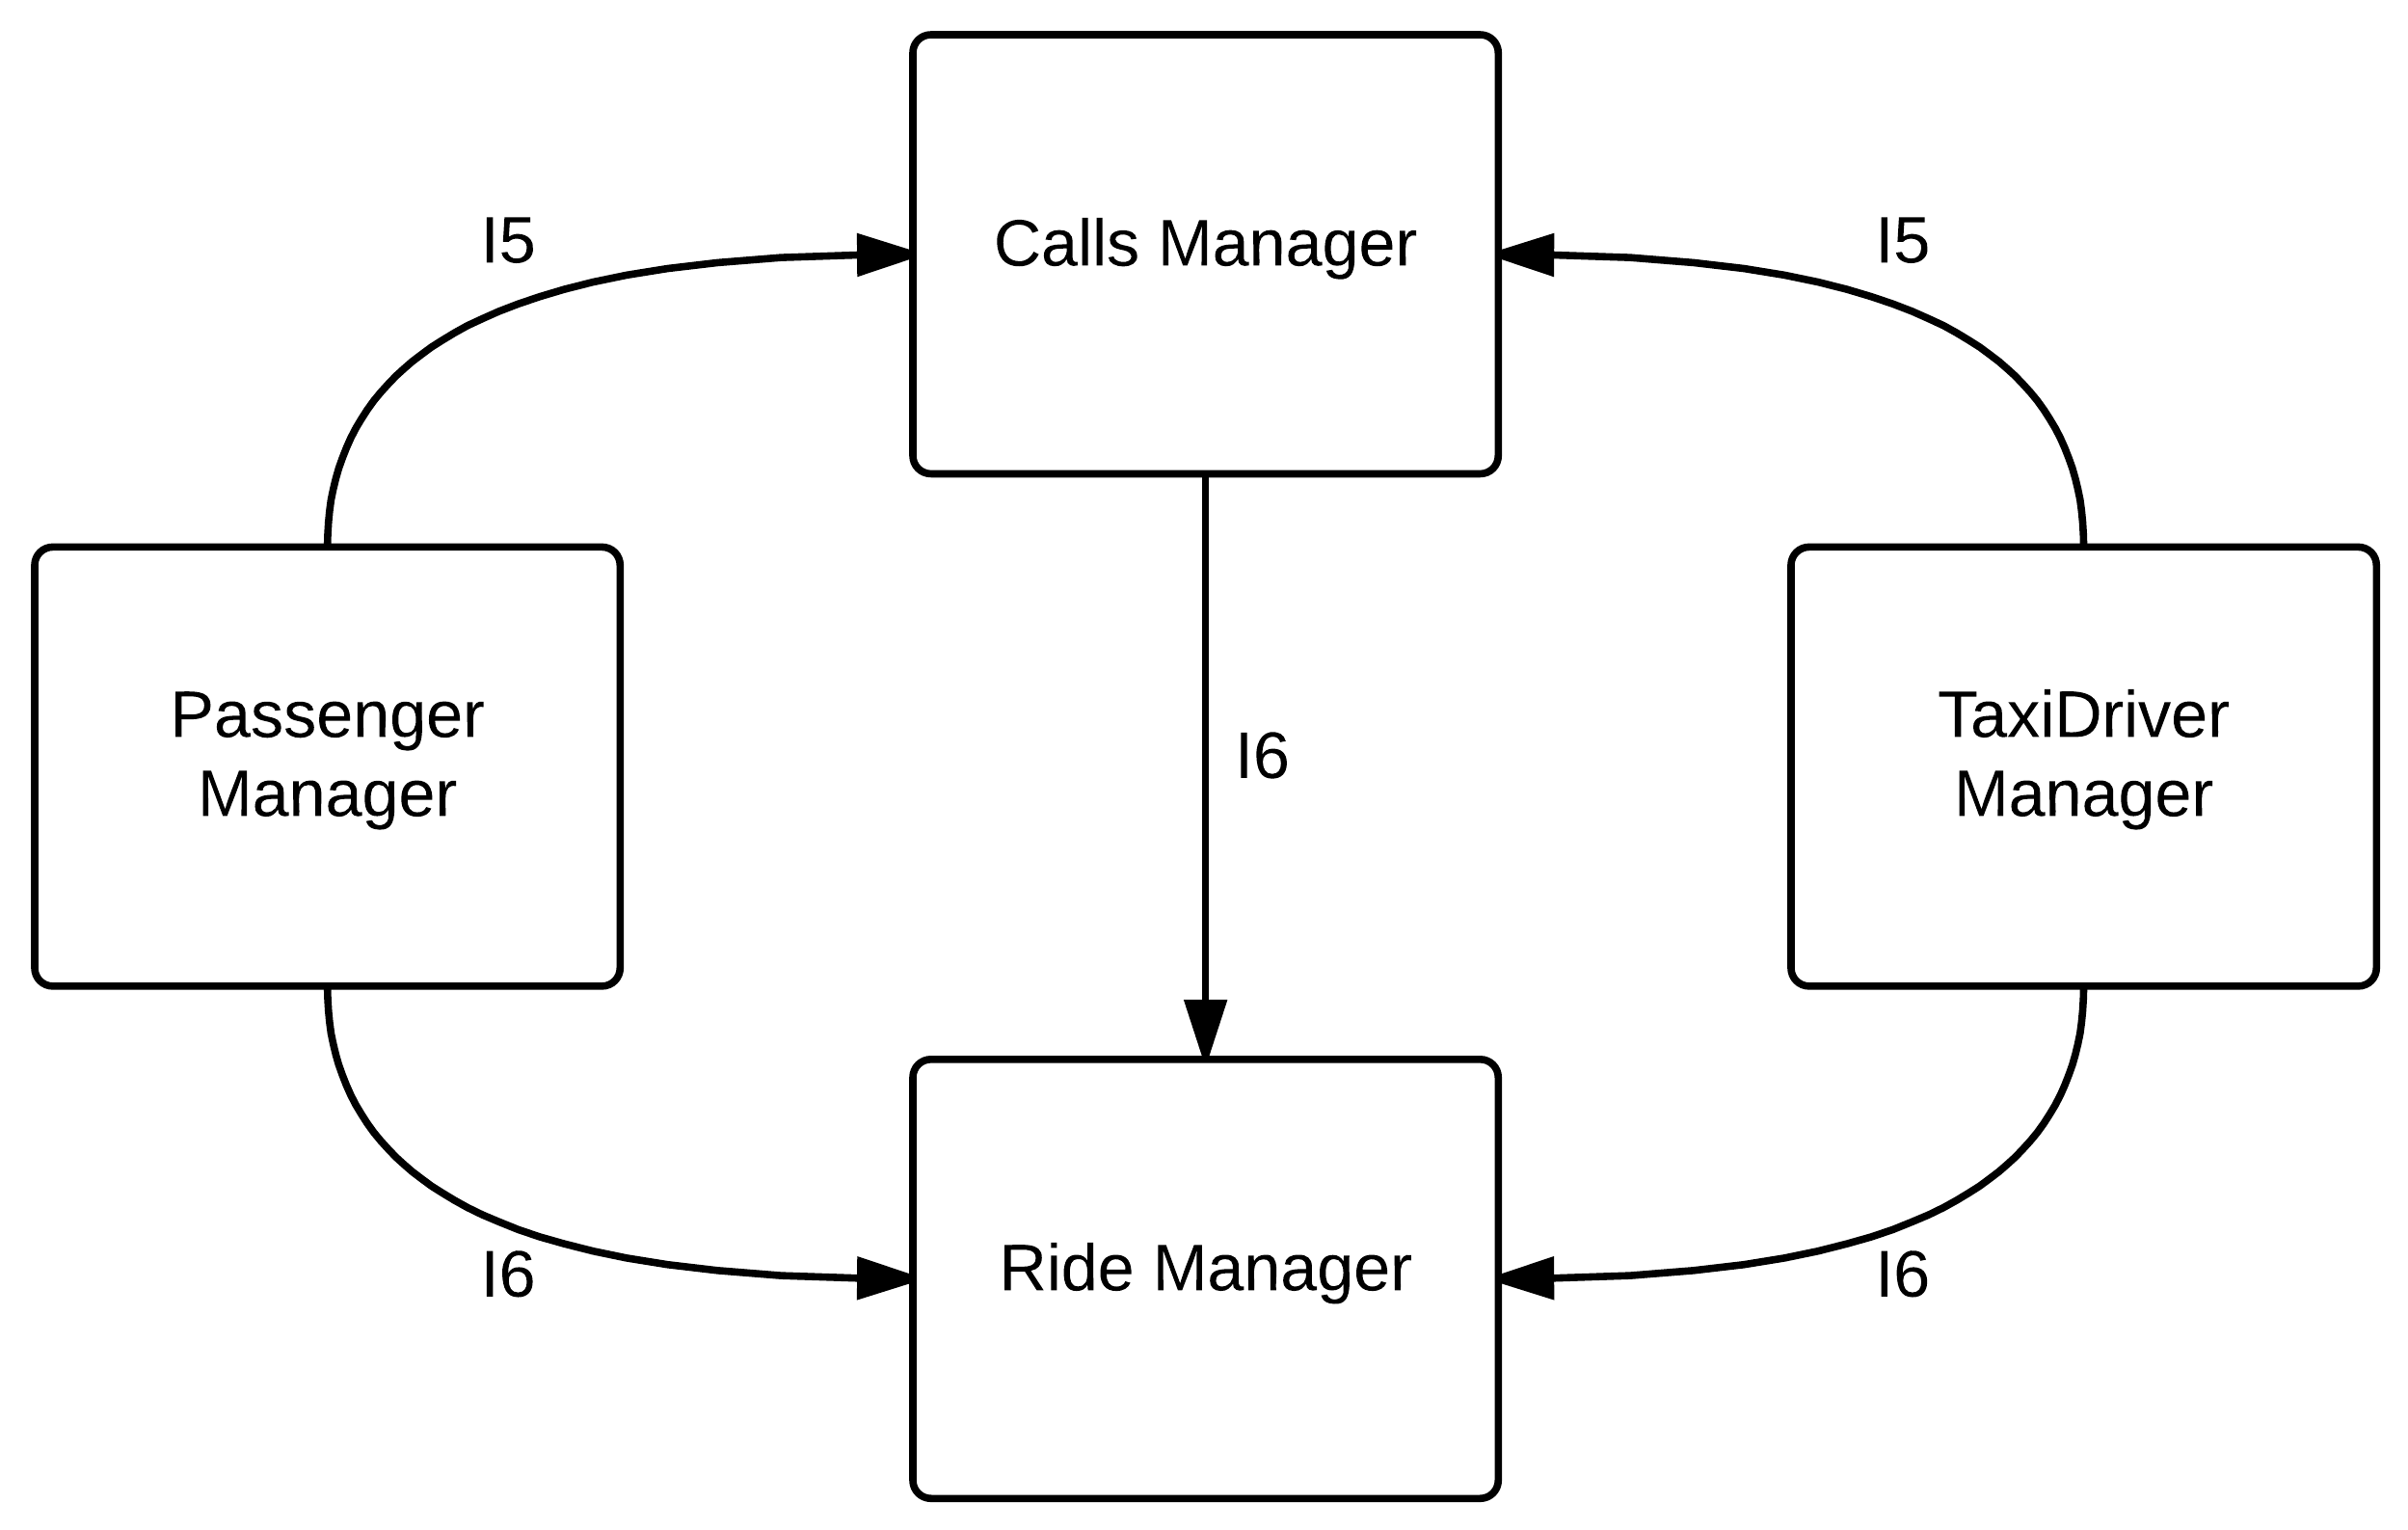
\includegraphics[width=\textwidth]{cpt/img/ITDPComponentDiagramsTP2}
\end{figure}

\begin{table}[!htbp]
\begin{center}
\begin{tabular}[t]{c|p{0.7\textwidth}|c}

\textbf{ID} & \textbf{Integration Test} & \textbf{Paragraphs} \\
\hline
I5 & Passenger Manager, TaxiDriver Manager $\rightarrow$ Calls Manager & 3.1.5  3.2.2\\
\hline
I6 & Passenger Manager, TaxiDriver Manager, Calls Manager $\rightarrow$ Ride Manager & 3.1.6  3.2.2\\
\hline
\end{tabular}
\end{center}
\end{table}
\clearpage

\begin{figure}[!htbp]
\centering
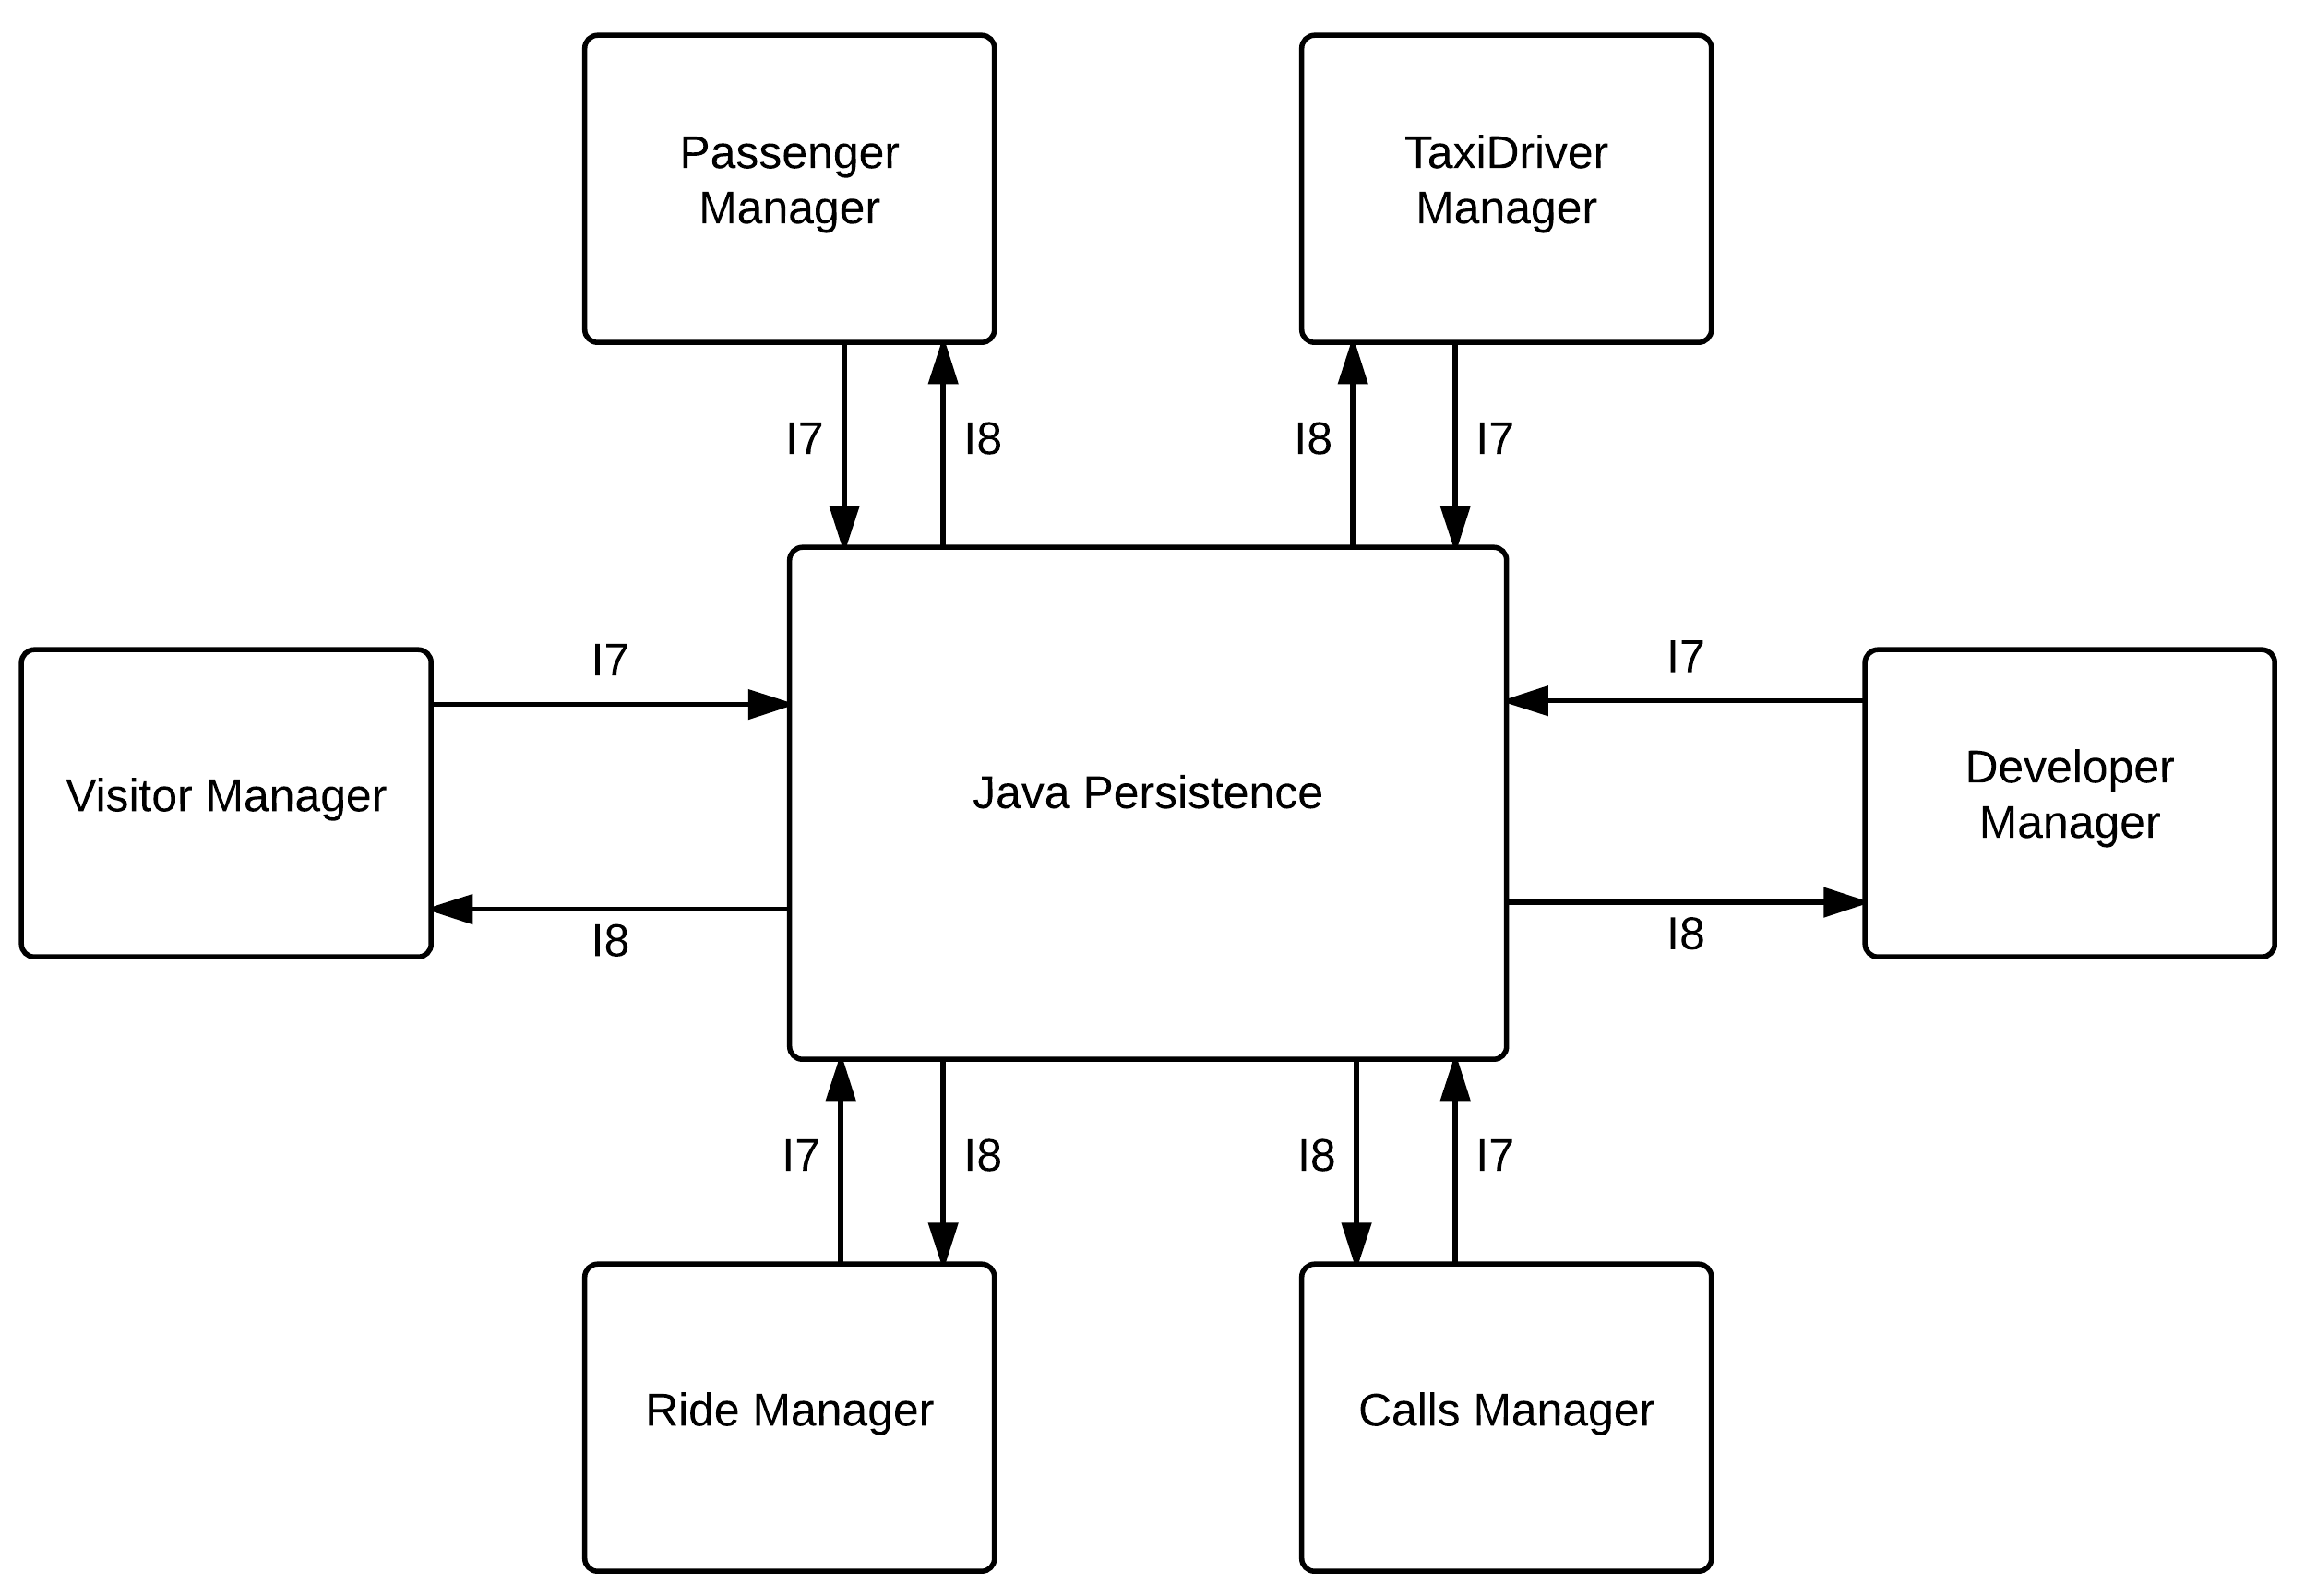
\includegraphics[width=\textwidth]{cpt/img/ITDPComponentDiagramsTP3}
\end{figure}

\begin{table}[!htbp]
\begin{center}
\begin{tabular}[t]{c|p{0.7\textwidth}|c}

\textbf{ID} & \textbf{Integration Test} & \textbf{Paragraphs} \\
\hline
I7 & Visitor Manager, Passenger Manager, TaxiDriver Manager, Developer Manager, Calls Manager, Ride Manager $\rightarrow$ Java Persistence & 3.1.7  3.2.3 \\
\hline
I8 & Java Persistence $\rightarrow$ Visitor Manager, Passenger Manager, TaxiDriver Manager, Developer Manager, Calls Manager, Ride Manager & 3.1.8  3.2.3 \\
\hline
\end{tabular}
\end{center}
\end{table}
\clearpage

\begin{figure}[!htbp]
\centering
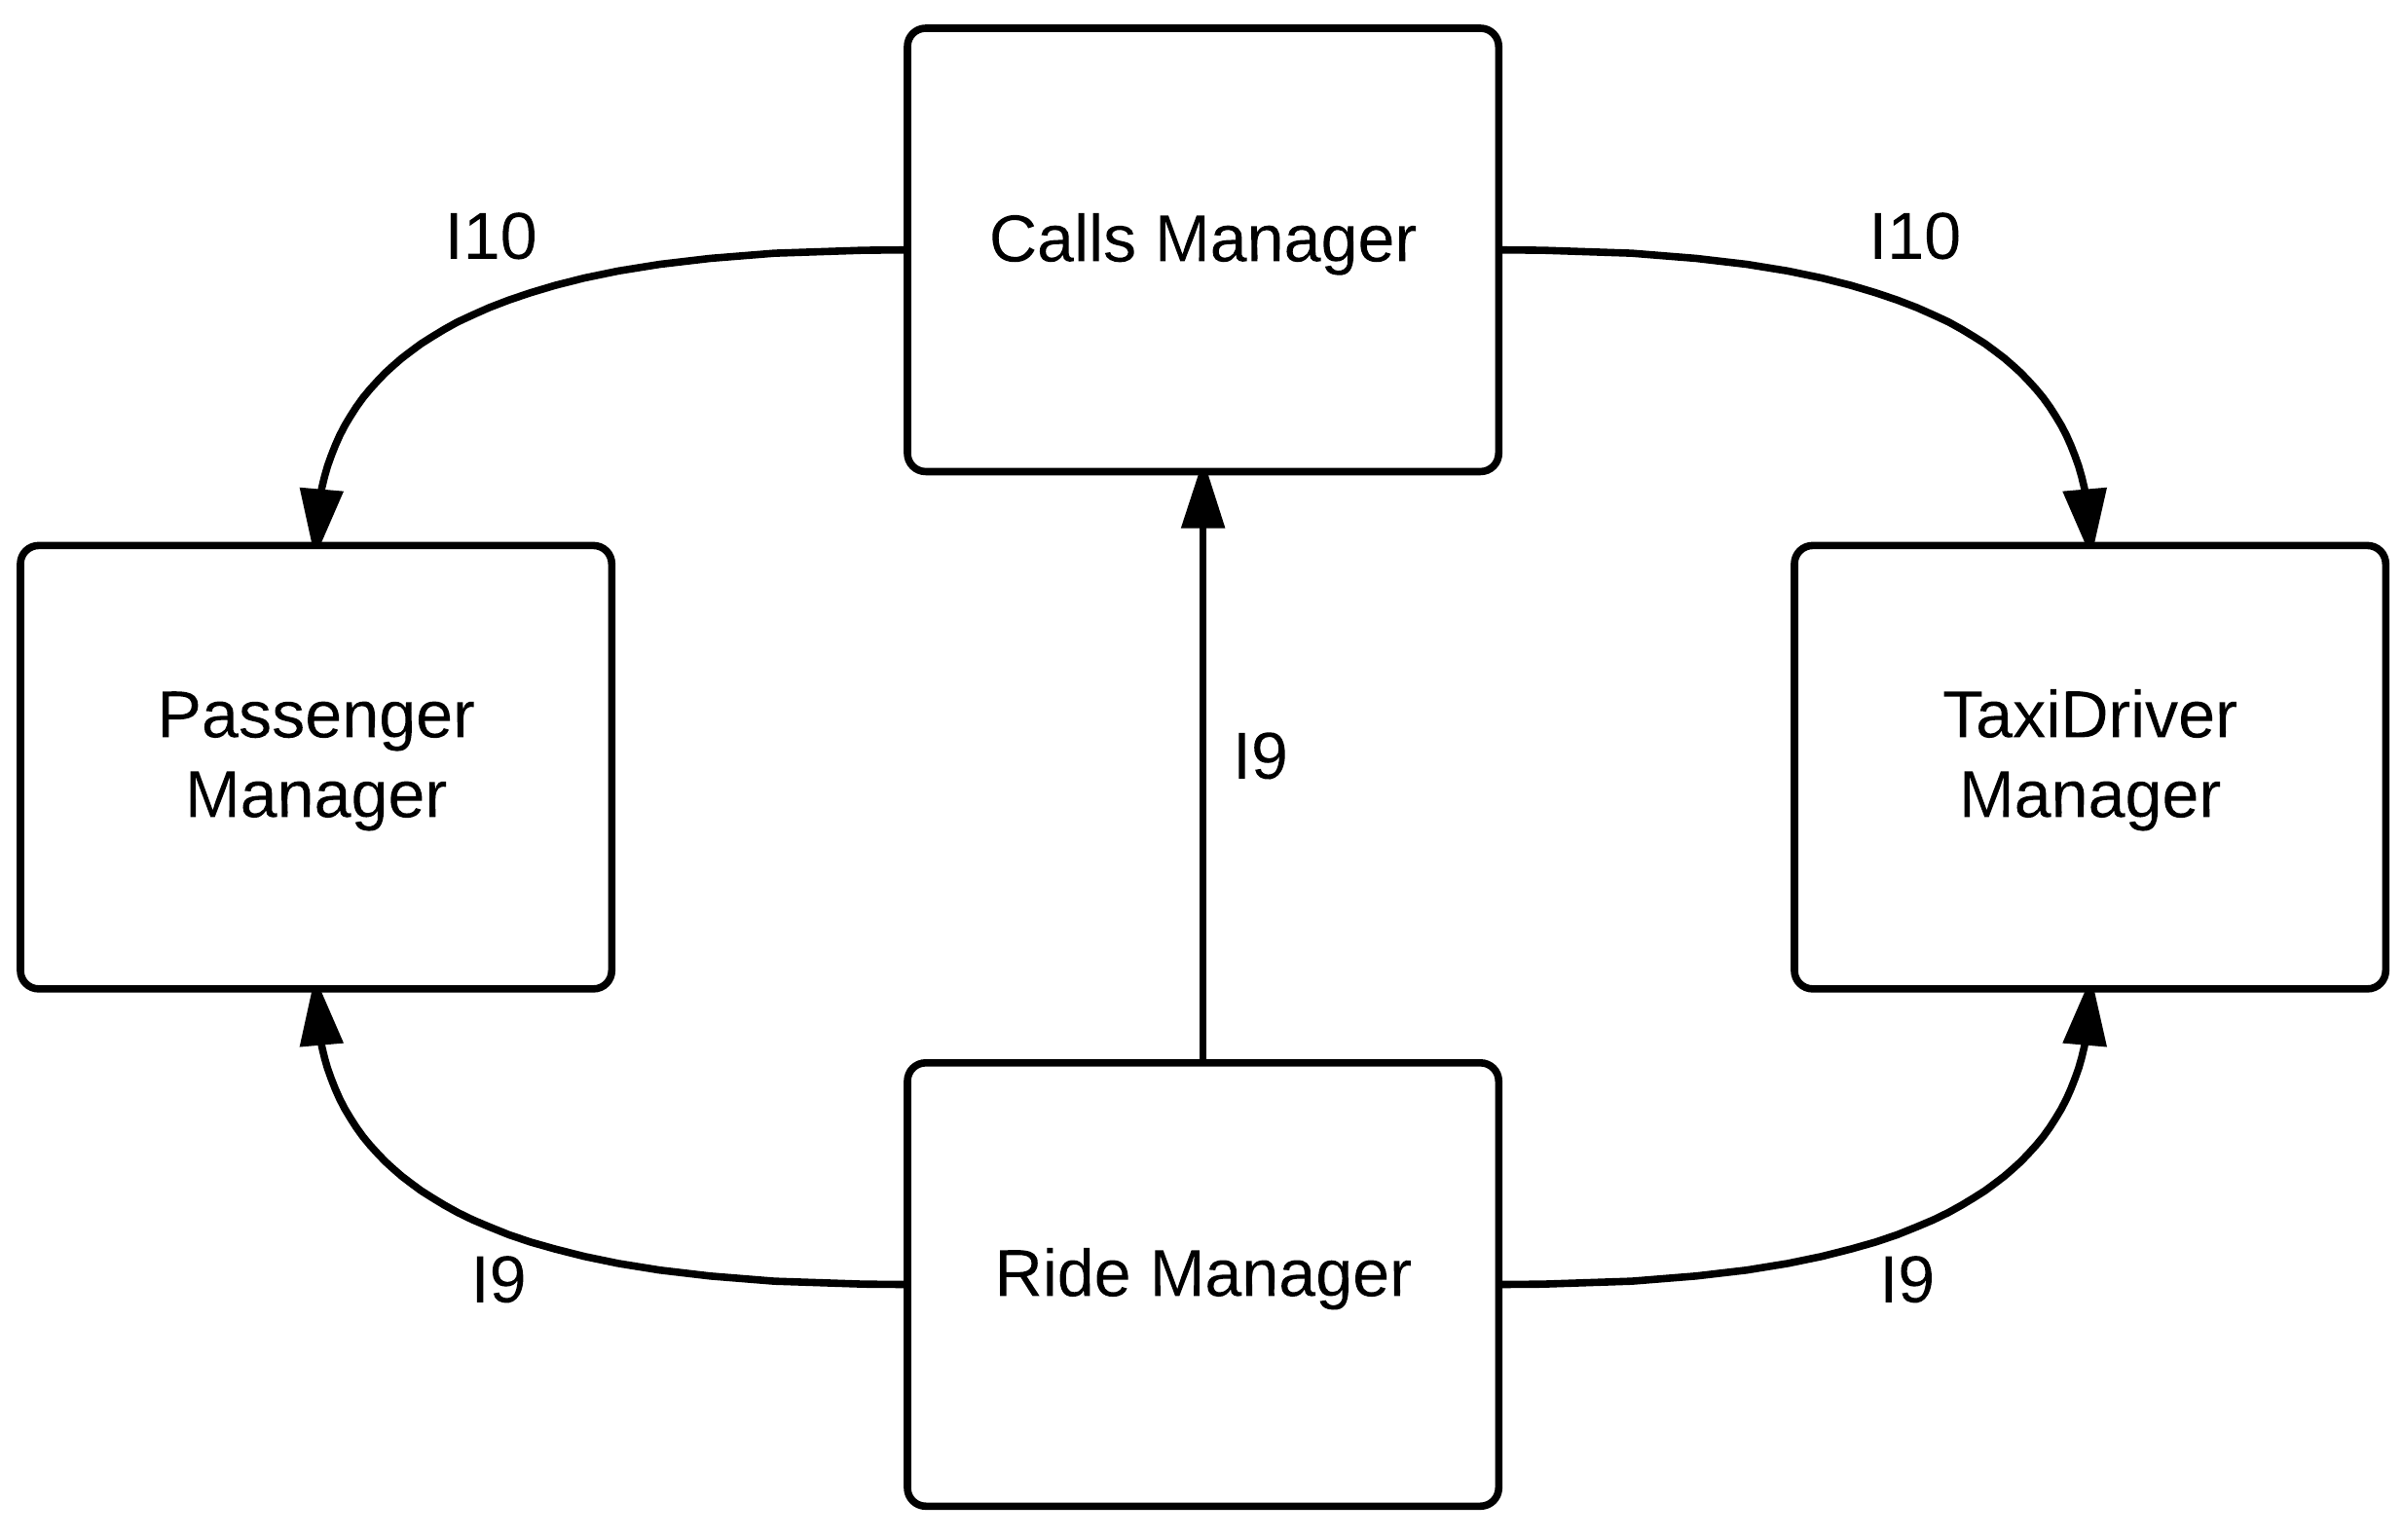
\includegraphics[width=\textwidth]{cpt/img/ITDPComponentDiagramsTP4}
\end{figure}

\begin{table}[!htbp]
\begin{center}
\begin{tabular}[t]{c|p{0.7\textwidth}|c}

\textbf{ID} & \textbf{Integration Test} & \textbf{Paragraphs} \\
\hline
I9 &  Ride Manager $\rightarrow$ Passenger Manager, TaxiDriver Manager, Calls Manager & 3.1.9  3.2.4\\
\hline
I10 & Calls Manager $\rightarrow$ Passenger Manager, TaxiDriver Manager & 3.1.10  3.2.4\\
\hline
\end{tabular}
\end{center}
\end{table}
\clearpage

\begin{figure}[!htbp]
\centering
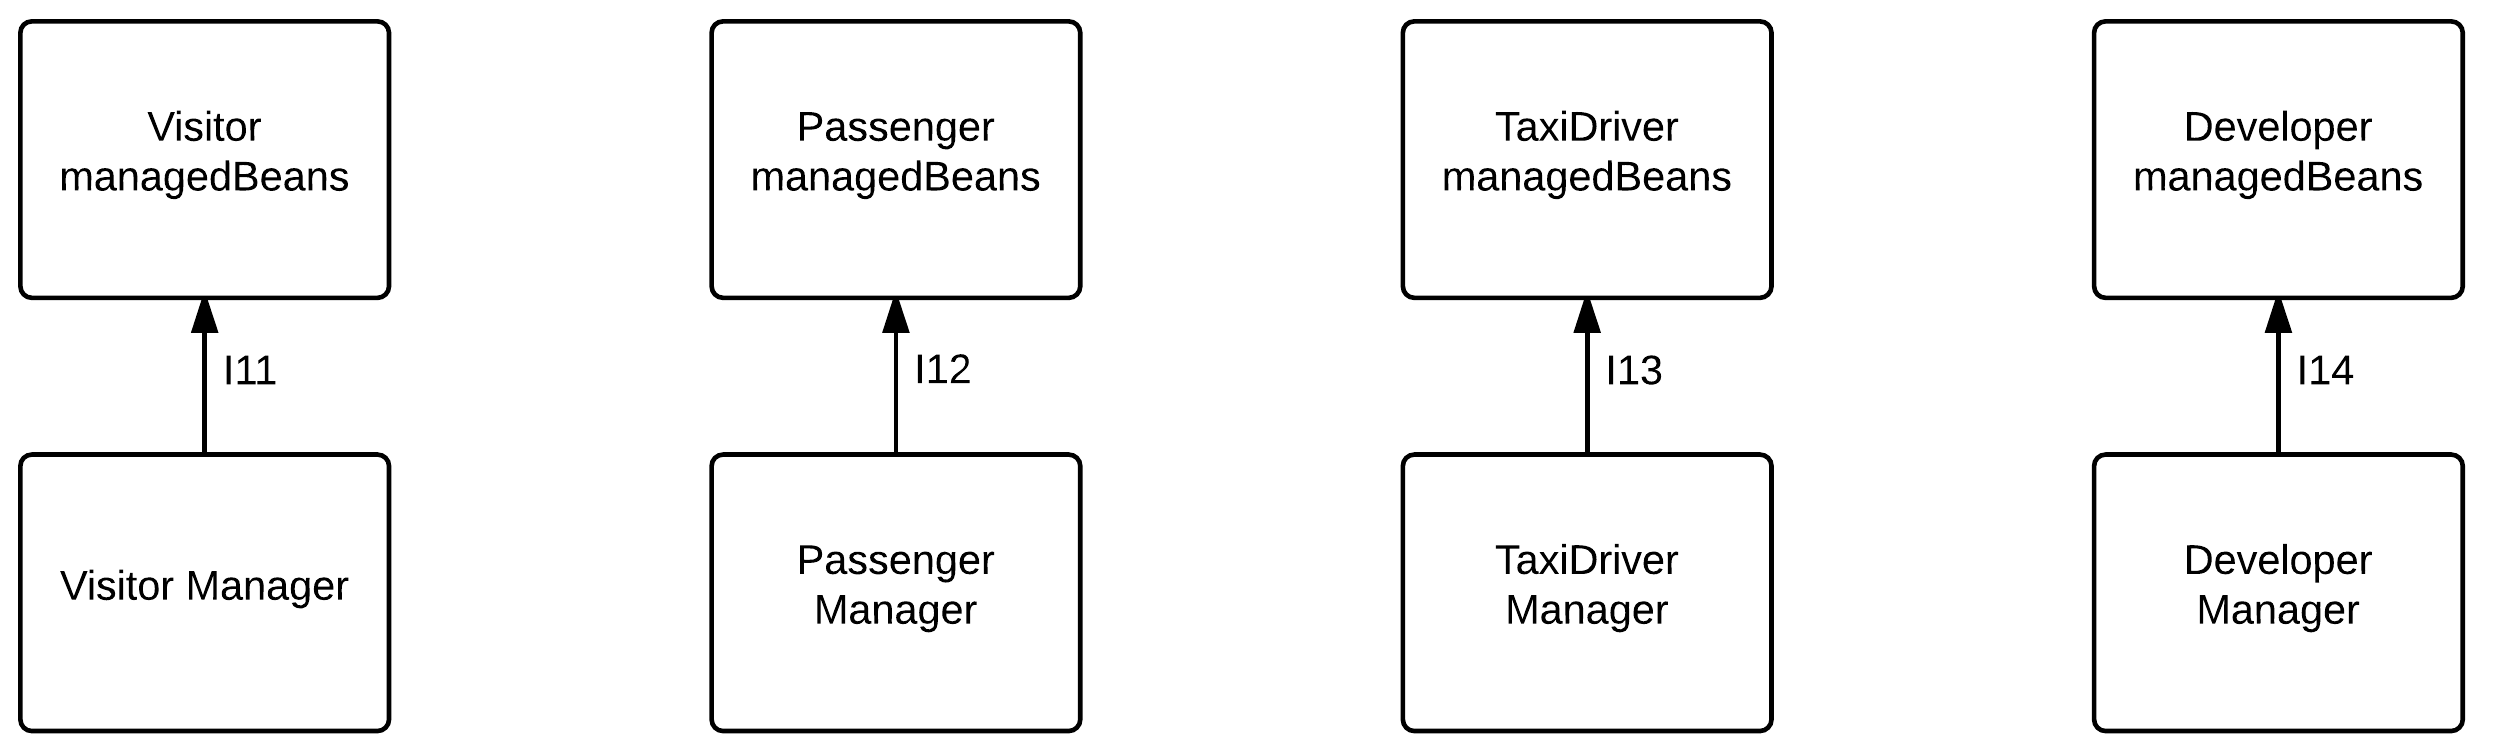
\includegraphics[width=\textwidth]{cpt/img/ITDPComponentDiagramsTP5}
\end{figure}

\begin{table}[!htbp]
\begin{center}
\begin{tabular}[t]{c|p{0.7\textwidth}|c}

\textbf{ID} & \textbf{Integration Test} & \textbf{Paragraphs} \\
\hline
I11 & Visitor Manager $\rightarrow$ Visitor managedBean & 3.1.11  3.2.5 \\
\hline
I12 & Passenger Manager $\rightarrow$ Passenger managedBean & 3.1.12  3.2.5 \\
\hline
I13 & TaxiDriver Manager $\rightarrow$ TaxiDriver managedBean & 3.1.13  3.2.5 \\
\hline
I14 & Developer Manager $\rightarrow$ Developer managedBean & 3.1.14  3.2.5 \\
\hline

\end{tabular}
\end{center}
\end{table}
\clearpage